\subsection{Subgradiente}

Las funciones convexas poseen algunas propiedades usuales de diferenciabilidad, y una de ellas es la existencia de la derivada direccional 
lateral (derecha e izquierda) en toda direcci\'on en un punto interior de su dominio, as\'i como en el caso usual de la derivada direccional 
de una funci\'on diferenciable puede ser escrita en t\'erminos del vector gradiente, que est\'a asociado con un hiperplano tangente al
gr\'afico de la funci\'on, la derivada lateral derecha de una funci\'on convexa, no necesariamente diferenciable puede ser escrita en
t\'erminos de vectores subgradientes que est\'an asociados con hiperplanos soportes al epigrafo de la funci\'on. En lo sucesivo nos 
referiremos a la derivada direccional derecha como derivada direccional \cite{navarro}.
\medskip

{\definicion Sean $f: \mathbb{R}^n \longmapsto \mathbb{R},\, x\in \mathbb{R}^n;$ la derivada direccional de $f$ en $x$ con respecto a
$y$ es definida como el siguiente lı\'imite:


\[f'(x) = \displaystyle{\lim_{t \rightarrow 0^{+} }\dfrac{f(x + ty)- f(x)}{t}}\]

si este l\'imite existe. \label{derivada-dir}}\\

%------------------------------------epigrafo e hipografo----------------------------------------------------------

\textbf{\large Hipografo y epigrafo de una funci\'on}
\medskip

Una funci\'on $f$ en $S$ puede ser completamente descrita por el conjunto $\{[x, f(x)]:\, x \in S\} \subset \mathbb{R}^n,$ cada cual se 
refiere \textbf{\itshape grafo} de la funci\'on. Se puede construir uno de dos conjuntos que est\'an relacionados al grafo de la funci\'on 
$f:$ el {\it epigrafo} y el {\it hipografo} de $f.$
\medskip

{\definicion Sea $S$ un conjunto no vac\'io en $\mathbb{R}^n,$ y sea $f: S \longmapsto \mathbb{R}.$ El epigrafo de $f$ denotado por 
{\it epi(f),} es un subconjunto de $\mathbb{R}^{n+1}$ definido por:
$$\{(x, y):\, x \in S,\,  y \in \mathbb{R},\, y \geqslant f(x)\}$$

El {\it hipografo} de $f$ denotado por {\it hyp(f)} es un subconjunto de $\mathbb{R}^{n+1}$ definido por:
$$\{(x, y):\, x \in S,\, y \in \mathbb{R},\, y \leqslant f(x)\}$$  \label{epi-hipo}}

\begin{figure}
   \centering
   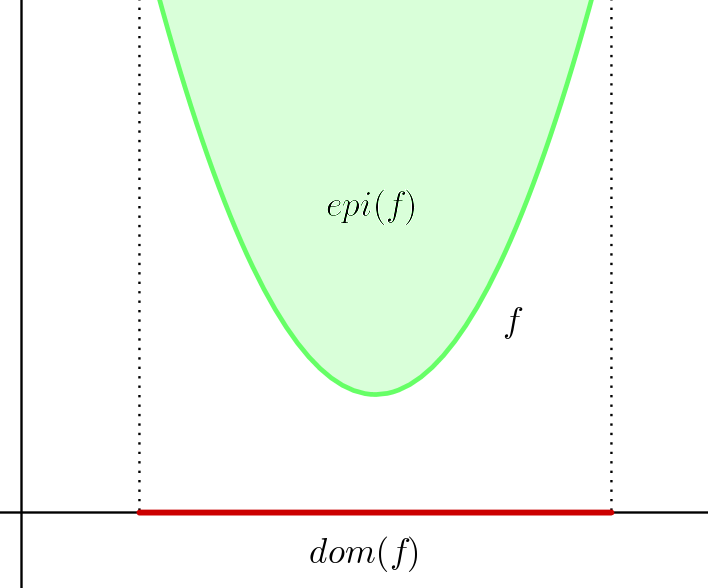
\includegraphics{./partes/sub_sec/codigo-image/epi.png}
   \caption{Epigrafo de una funci\'on $f$ en $\mathbb{R}$ \cite{lara}}
\end{figure}

{\teorema Sea $S$ un conjunto convexo no vac\'io en $\mathbb{R}^n,$ y sea $f: S \longmapsto \mathbb{R}.$ Entonces $f$ es convexa si y solo si
el $epi(f)$ es un conjunto convexo.\label{epi-convx}} \medskip


%-------------------------------------fin de epi e hipo------------------------------------------------------------

{\definicion Sean $f: \mathbb{R}^n \longmapsto \mathbb{R},\,\, x_0 \in \mathbb{R}^n$ Un vector $\vec{s} \in \mathbb{R}^n$ tal que:
$$f(x) \geqslant f(x_{0}) + \langle s, x - x_0 \rangle,\,\, \forall x\in \mathbb{R}^n$$

es llamado un subgradientede $f$ en $x_0$ \cite{navarro}  \label{subgradiente}}\\

El conjunto de subgradientes de una funci\'on $f$ en el punto $x_0$ es llamado subdiferencial de $f$ en $x_0$ y se denota por 
$\partial f(x_0).$
\medskip

{\definicion Si $\partial f(x_0) \neq \emptyset$ diremos que $f$ es diferenciable en $x_0.$ \label{sub-dif}}\\


Geom\'etricamente, $s \in \mathbb{R}^n$ es un subgradiente de la funci\'on convexa $f$ en $x_0$ si el gr\'afico de $f$ en $\mathbb{R}^{n+1}$
est\'a por encima del gr\'afico del hiperplano $y = f(x) + \langle s, x - x_0 \rangle .$ Como $(x_0, f(x_0))$ est\'a en el hiperplano, este 
hiperplano constituye un hiperplano soporte a $epi(f)$ en $(x_0, f(x_0)).$ Esto es, la existencia de un vector subgradiente establece la
existencia de un hiperplano soporte no vertical a $epi(f)$ en $(x_0, f(x_0)).$

\begin{figure}
   \centering
   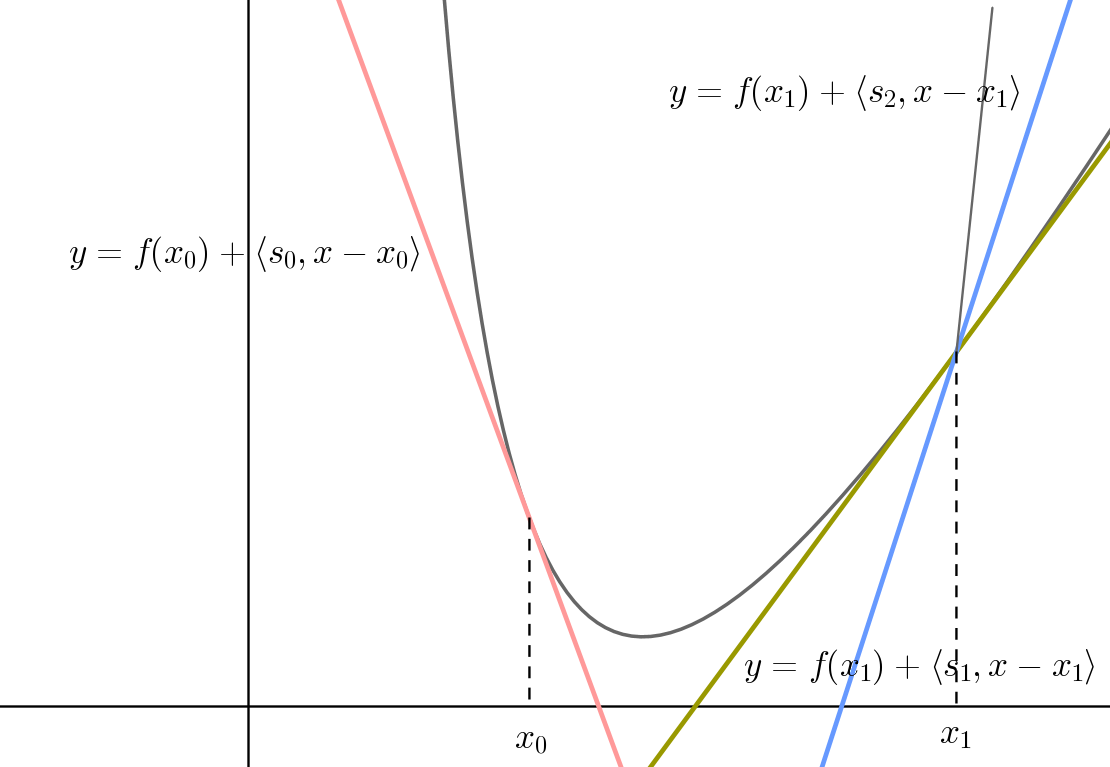
\includegraphics{./partes/sub_sec/codigo-image/subgradiente.png}
   \caption{Interpretaci\'on geom\'etrica del subgradiente en $\mathbb{R}$ \cite{navarro}}
\end{figure}

El siguiente teorema establece que toda funci\'on convexa es subdiferenciable en el interior de su dominio \cite{navarro}.

{\teorema Sea $f$ una funci\'on convexa definida en un convexo $S,$ entonces en cada punto $x_0 \in \mathring{S}$ se tiene que
$\partial f(x_0) \neq \emptyset$ \label{convx-int}}
\medskip

El rec\'iproco del teorema anterior es falso, pues la condici\'on de ser punto interior es indispensable, por ejemplo, si se considera la
funci\'on convexa $f:[0, \infty ) \longmapsto \mathbb{R}$ dada por $f(x) = - \sqrt{x}$ entonces se tiene que $\partial f(0) = \emptyset$
\newpage







